\textbf{\Huge{Diplomarbeitsdokumentation}}

\begin{tabular}{|m{4.5cm}|m{9cm}|}															%senkrechter Strich steht f�r horizontale Linien
																																%mit m k�nnen die Gr��en der Zellen bestimmt werden
		\hline																											% \hline f�r eine horizontale Linie in der Tabelle
		& \\																												% mit & werden die Zellen abgerentzt
		Verfasser & Felix Sandri, Philipp Kaltenleitner, \\	% \\ steht f�r einen Zeilenumbruch in einer Tabelle
							& Mert G�rel, David Petrovic  \\ 
		& \\				
		\hline
		& \\
		Jahrgang Schuljahr & 5BHET \\ & 2023/24  \\ 								
		& \\ 			
		\hline
		
		& \\
		Thema der & Entwicklung und Fertigung eines selbstfahrenden \\ 
		Diplomarbeit & Modelautos\\ 
		& \\ 
		\hline
		& \\
		Kooperationspartner & HTBLuVA Salzburg \\ 
												& Kyocera AVX \\
											  & Mean Well/ Pro Connect \\ 
												& WG Global GmbH\\
												& SDP Automobile\\	
												& Mario's Autoteile\\	
												& Innovation Salzburg Pioniergarage GmbH\\ 
												& Schraubenking GmbH\\	
												
		& \\
		\hline \hline
		
		& \\
		Aufgabenstellung & Das Ziel besteht darin, ein Modellauto zu entwickeln, welches auf dem Gel�nde der HTBLuVA Salzburg autonom fahren kann. Hierf�r wird ein Auto von Grund auf neu konstruiert, inklusive aller mechanischen, elektronischen und softwaretechnischen Komponenten. Des Weiteren soll das Fahrzeug in allen mechanischen und elektrotechnischen Aspekten voll funktionsf�hig sein.
		\\
		& \\ 
		\hline \hline
		& \\
		
		Realisierung & Um das autonome Fahren zu erm�glichen, wird ein vollst�ndig neues Fahrzeug mit allen erforderlichen mechanischen Komponenten entwickelt, das ausreichend Platz bietet, um s�mtliche Elektronik unterzubringen. Zur Umgebungserfassung nutzt Athena einen LiDAR-Sensor sowie acht weitere Ultraschallsensoren. Die Hauptrecheneinheit ist ein Lattepanda 3 Delta, der zudem �ber eine Dual Edge TPU verf�gt, was eine schnellere Verarbeitung der Sensordaten erm�glicht. Durch k�nstliche Intelligenz kann Athena nicht nur die Daten verarbeiten, sondern auch das Fahrzeug steuern. Zus�tzlich wird ein ESP32 als Sub-Prozessor verwendet.\\
		 
		& \\ 
		\hline
		
		\end{tabular}	
		
		\pagebreak
				
		\begin{tabular}{|m{4.5cm}|m{9cm}|}
		
		\hline
		& \\
		Abbildung & 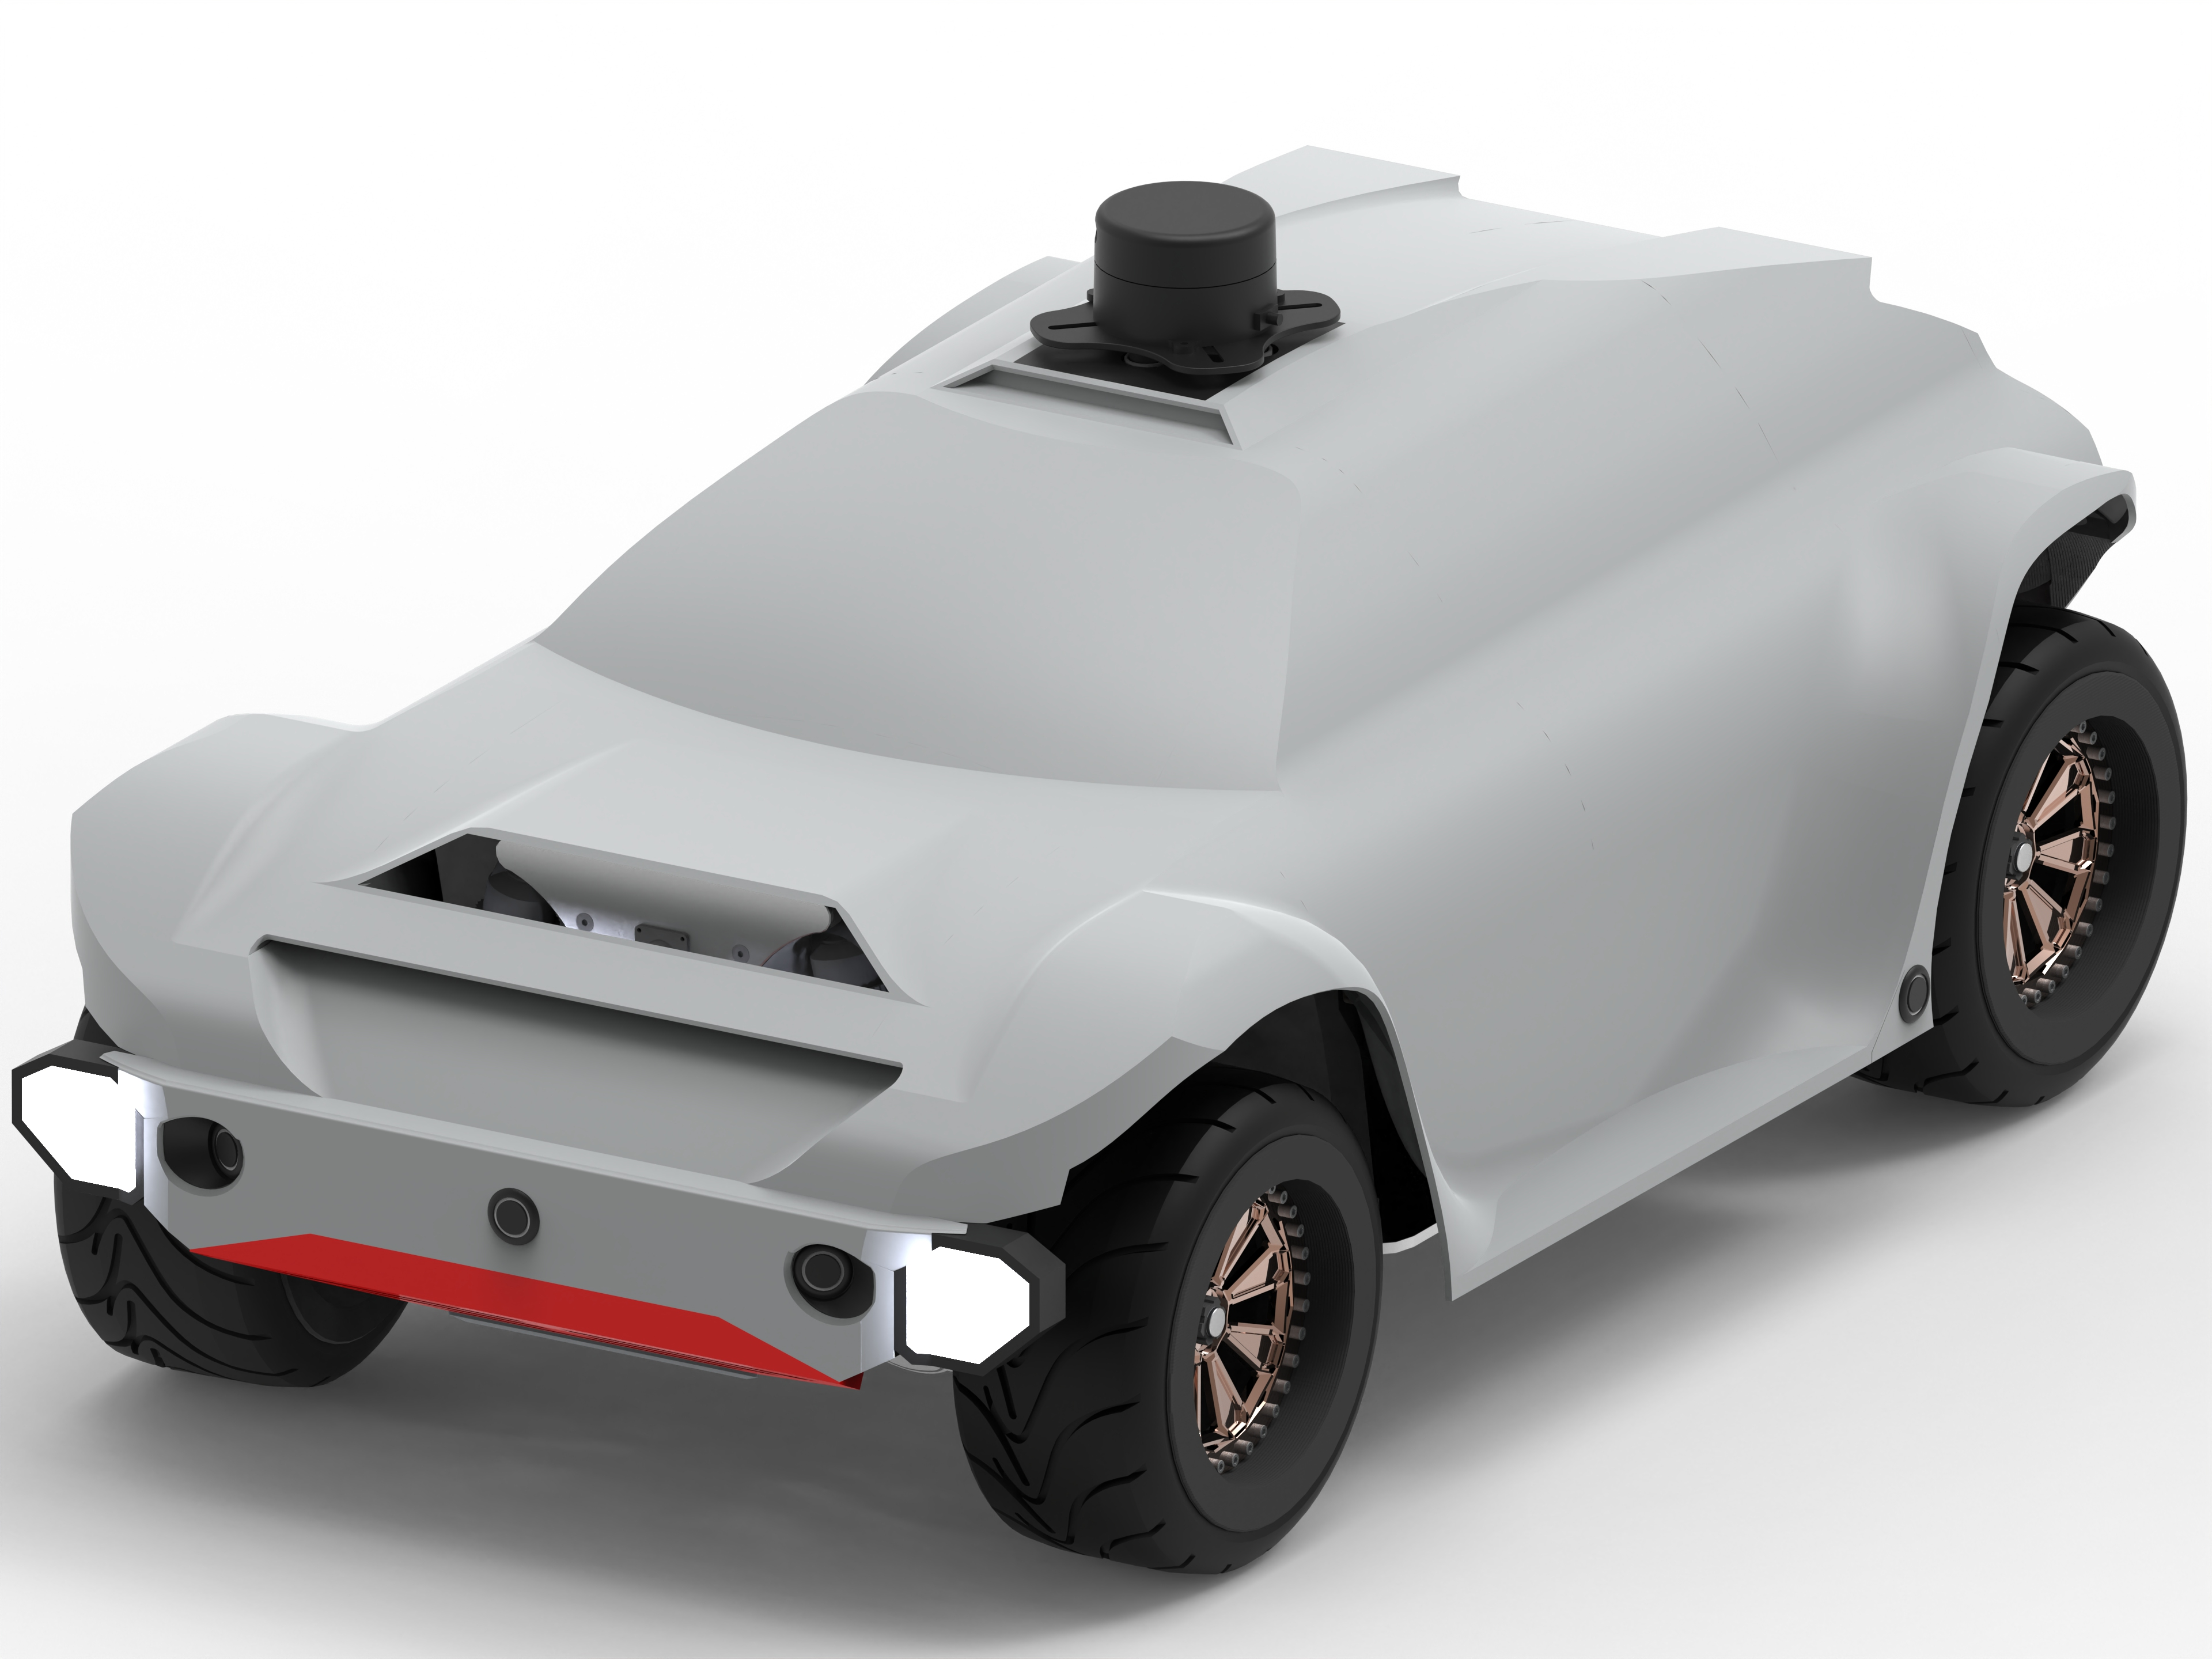
\includegraphics[width=8.5cm]{./4_Mechanik/Abbildungen/Aufbau_Anleitung_render/Athena_fertig_4}\\ 
		& \\
		\hline 
	
		\end{tabular}	
		
		\begin{tabular}{|m{4.5cm}|m{9cm}|}
		
		\hline
		Ergebnisse & Das Modellauto Athena wurde sowohl mechanisch als auch in Bezug auf Hardware und Software rechtzeitig fertiggestellt und erfolgreich in Betrieb genommen. \\ 
		\hline
		
		\end{tabular}
		
		\begin{tabular}{|m{4.5cm}|m{9cm}|}\hline
		
		M�glichkeit der Einsichtnahme in die Arbeit & Die Diplomarbeit ist in gebundener Form in der
																									Schulbibliothek als auch bei AV Prof. Dipl-Ing.
																									(FH) Roland Holzer einzusehen. Dar�ber hinaus besitzt
																									jedes Mitglied des Projektteams eine vollst�ndige Version 
																									in gebundener und digitaler Form. \\ 
		\hline  
		
		\end{tabular}
		
		\begin{tabular}{|m{4.5cm}|m{4.28cm}|m{4.28cm}|}	%letzte Zeile muss in 3 Spalten unterteilt werden
		
		\hline
		
		Approbation & Pr�fer/Pr�ferin & Abteilungsvorstand \\ 
		(Datum/Unterschrift) &  & 	\\  
		&	& \\ 
		\hline

		\end{tabular}					%Ende der Tabelle
		\newpage
		
		
		
		
		
		
		
		\textbf{\Huge{Diploma Thesis Documentation}}

\begin{tabular}{|m{4.5cm}|m{9cm}|}															%senkrechter Strich steht f�r horizontale Linien
																																%mit m k�nnen die Gr��en der Zellen bestimmt werden
		\hline																											% \hline f�r eine horizontale Linie in der Tabelle
		& \\																												% mit & werden die Zellen abgerentzt
		Authors & Felix Sandri, Philipp Kaltenleitner, \\	% \\ steht f�r einen Zeilenumbruch in einer Tabelle
							& Mert G�rel, David Petrovic  \\
		& \\				
		\hline
		& \\
		Form Academic year & 5BHET \\ & 2023/24  \\ 								
		& \\ 			
		\hline
		
		& \\
		Topic & Development and Manufacturing of a Self-Driving\\ 
					& Model Car\\ 
		& \\ 
		
		\hline
		
		& \\
		Co-operation  			& HTBLuVA Salzburg \\ 
												& Kyocera AVX \\
											  & Mean Well/ Pro Connect \\ 
												& WG Global GmbH\\
												& SDP Automobile\\	
												& Mario's Autoteile\\	
												& Innovation Salzburg Pioniergarage GmbH\\ 
												& Schraubenking GmbH\\	
												
		& \\
		\hline \hline
		& \\
	Assignment of Tasks & The goal is to develop a model car capable of autonomous driving on the premises of HTBLuVA Salzburg. To achieve this, a car will be completely designed from scratch, including all mechanical, electronic, and software components. Furthermore, the vehicle is intended to be fully functional in all mechanical and electrical aspects. \\
		& \\ 
		\hline \hline
		& \\
		 
		Realization & To enable autonomous driving, a completely new vehicle is being developed with all necessary mechanical components, providing ample space to accommodate all electronics. Athena utilizes a LiDAR sensor and eight additional ultrasonic sensors for environment mapping. The main computing unit is a Lattepanda 3 Delta, equipped with a Dual Edge TPU for faster sensor data processing. Through artificial intelligence, Athena can not only process data but also control the vehicle. Additionally, an ESP32 is used as a sub-processor. \\
		 
		& \\ 
		\hline
		
		\end{tabular}	
		
		\begin{tabular}{|m{4.5cm}|m{9cm}|}
		
		\hline
		
		& \\
		Illustrative Graph & 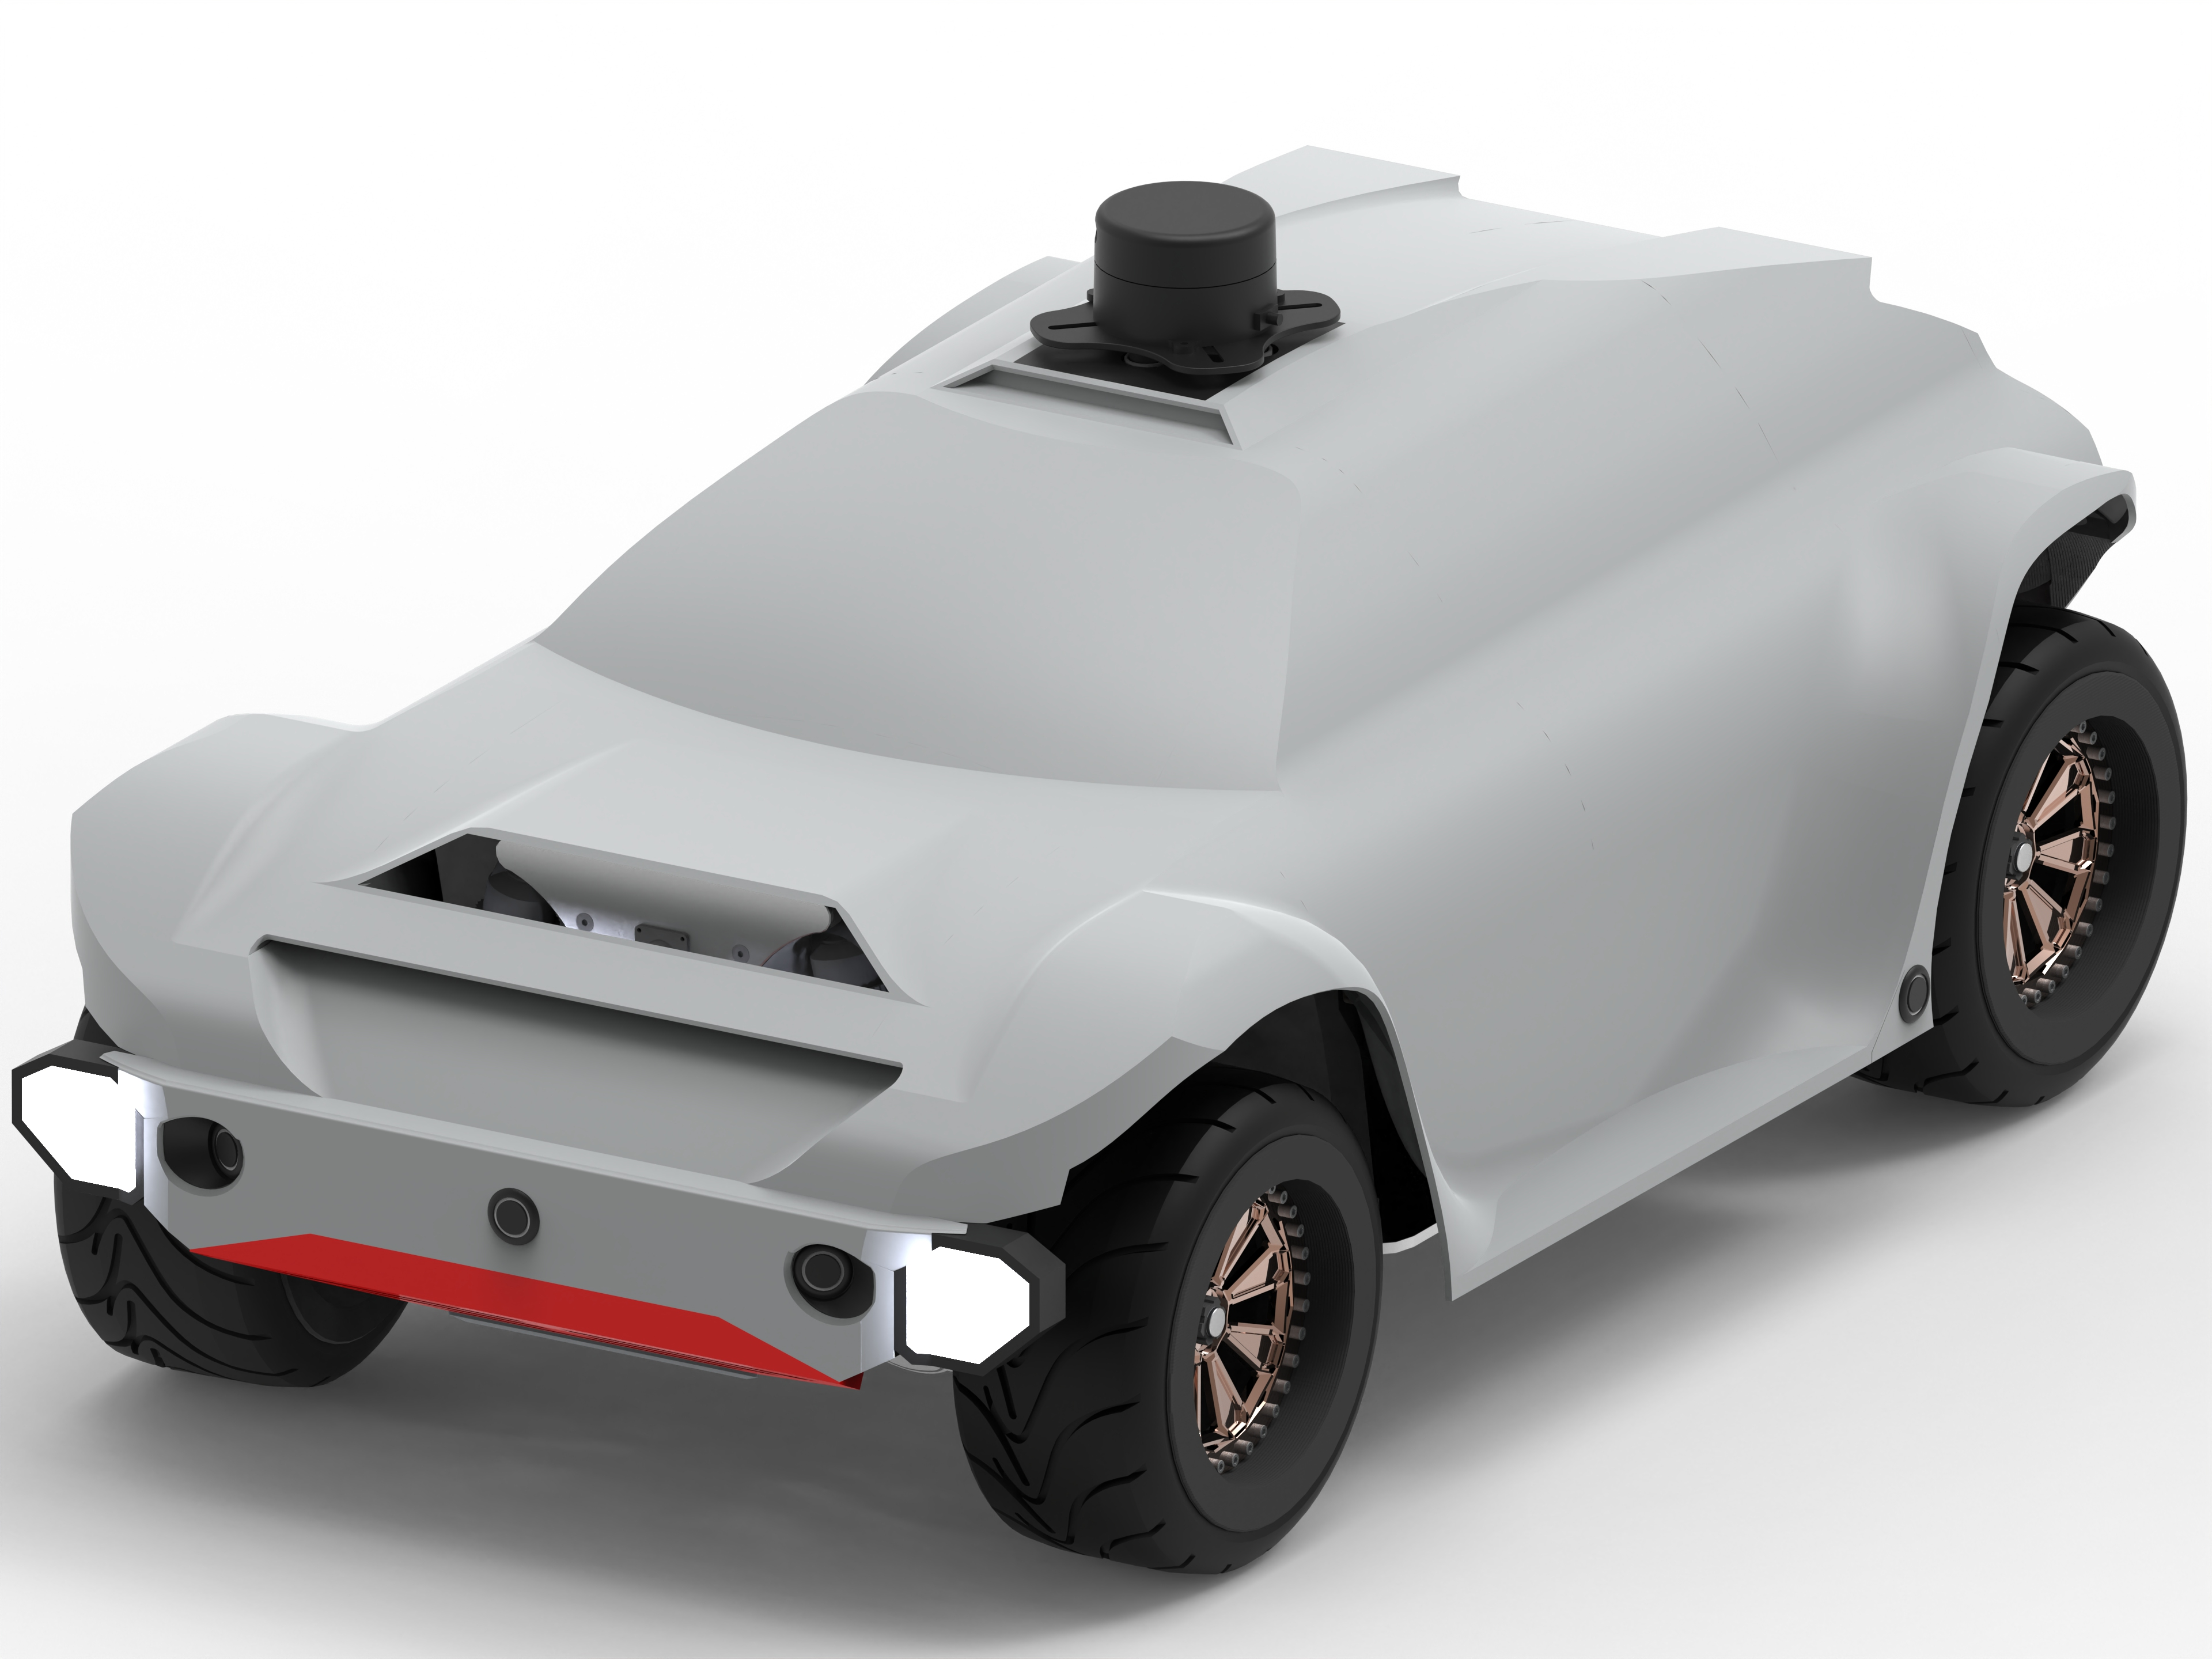
\includegraphics[width=8.5cm]{./4_Mechanik/Abbildungen/Aufbau_Anleitung_render/Athena_fertig_4}\\ 
		& \\
		
		\hline 
	
		\end{tabular}	
		
		\begin{tabular}{|m{4.5cm}|m{9cm}|}
		
		\hline
		Results & The model car Athena has been completed on time, both mechanically and in terms of hardware and software, and has been successfully put into operation. \\ 
		\hline
		
		\end{tabular}
		
		\begin{tabular}{|m{4.5cm}|m{9cm}|}\hline
		
		Accessibility of \newline Diploma Thesis	 		& 		The diploma thesis is available in the school library
																												as well as in the office of the head of department
																												Prof. Dipl-Ing. (FH) Roland Holzer. In addition,
																												each member of the project team has a complete
																												version in hardcover and digital form.\\ \hline  
		
		\end{tabular}
		
		\begin{tabular}{|m{4.5cm}|m{4.28cm}|m{4.28cm}|}	%letzte Zeile muss in 3 Spalten unterteilt werden
		
		\hline
		Approval & Examiner & Head of department \\ 
		(Date/Sign) &  & 	\\  
		& & \\ 
		\hline
		\end{tabular}					%Ende der Tabelle
		\newpage